% compress makes nav-bars as small as possible
% usenamse & dipsnames are xcolor options
\documentclass[compact, usenames, dvipsnames]{beamer}

% increase number of registers - don't move this!
\usepackage{etex}

% some smaller fixes for LaTeX2e
\usepackage{fixltx2e}

% Set language and encoding
\usepackage[T1]{fontenc}
\usepackage[utf8x]{inputenc}
\usepackage[english]{babel}

% Set font
\usepackage{palatino}
%\usepackage{bookman}
%\usepackage{utopia}
%\usepackage{times}
%\usepackage{newcent}
%\usepackage{charter}
%\usepackage{avant} 
%\usepackage{chancery}
%\usepackage{euler}
%\usepackage{lmodern}
\usepackage{subcaption}
%\usepackage[round]{natbib}

% General Style
%\usepackage[usenames,dvipsnames]{xcolor} % part of beamer
\usepackage{graphicx}
\usepackage{hyperref}
%\usepackage{paralist} !! Is incompatible with beamer class
\usepackage{mdframed}
\usepackage{jneurosci}
% All pictures in other folder

% Mathematics
\usepackage{amsmath}
\usepackage{amssymb}


% TikZ for more complex drawings
\usepackage{tikz}
\usetikzlibrary{arrows, patterns, automata, trees, positioning, calc,%
    shapes, %
    % used for curled brace
    decorations.pathreplacing}

% Set Beamer class specific stuff

% Improve spacing on frame titles
\setbeamertemplate{frametitle}{%
    %some top border
    \vspace{.6em}%
    \insertframetitle%
    }

% Set footer with title/section
\setbeamertemplate{footline}{%
    %some left border
    \hspace{3em}%
    % Insert subsection or section / title if not available
    \ifx\firstpage\empty
    \else
        \ifx\insertsubsection\empty%
            \ifx\insertsection\empty%
            \inserttitle%
            \else%
            \insertsection%
            \fi%
        \else%
            \insertsubsection%
        \fi%
        \hfill%
        \insertframenumber\,/\,\inserttotalframenumber%
    \fi
    %some right + bottom border
    \hspace{3em}%
    \vspace{3em}%
    }

% Create a frame with background color for intermissions / questions.
% Args:
%       1: color
%       2: content
\newcommand*{\colorframe}[2]{%
    \begingroup%
    \setbeamercolor{background canvas}{bg=#1}%
    \begin{frame}{}
        \color{black}\centering\Large #2
    \end{frame}%
    \endgroup%
    }


% Show next entry transparently
\setbeamercovered{transparent}

% no navigation symbols
\setbeamertemplate{navigation symbols}{}

% Set Colors
\usecolortheme{default}

\definecolor{UniRed}{RGB}{165,30,55}
\definecolor{UniGold}{RGB}{180,160,105}
\definecolor{UniGrey}{RGB}{50,65,75}
\definecolor{UzhBlue}{RGB}{0,40,165}
\definecolor{UzhGrey}{RGB}{163,173,183}
\definecolor{UzhOrange}{RGB}{220,96,39}

\setbeamercolor{structure}{fg=UzhBlue}
\setbeamercolor{titlelike}{fg=black}
\setbeamercolor{title}{fg=UzhBlue}
\setbeamercolor{subtitle}{fg=Black}
\setbeamercolor{frametitlelike}{fg=UzhBlue}
\setbeamercolor{frametitle}{parent=frametitlelike}
\setbeamercolor{framesubtitle}{parent=frametitle}
\setbeamercolor{mini frame}{parent=structure}
\setbeamercolor{sepline}{fg=UzhGrey, bg=UzhGrey}
\setbeamercolor{partpage}{fg=UzhBlue, bg=UzhGrey}
\setbeamercolor{normal text}{fg=UniGrey}
\setbeamercolor{itemize item}{fg=black}
\setbeamercolor{enumerate item}{fg=black}



%%%%%%%%%%%%%%%%%%%%%%%%%%%%%%%%%%%%%%%%%%%%%%%%%%%%%%%%%%%%%%%%%%%%%%%%%%%%%%%%


\title{Atomic Contact Energies}
\subtitle{Bioinformatics II}
\author{Adrian Gei{\ss}ler, Max Emil Sch{\"o}n}
\date{June 22, 2015}

\newcommand*{\ColorIntro}{Cerulean}
\newcommand*{\ColorMethod}{Lavender}%Rhodamine}
\newcommand*{\ColorResults}{YellowGreen}%LimeGreen}
\newcommand*{\ColorDiscussion}{Peach}

\begin{document}

    \newcommand*{\firstpage}{}
    \begin{frame}{}
        \titlepage%
        \centering%
        { Tutor: Linus Backert}
    \end{frame}
    \renewcommand*{\firstpage}{non-empty string to start showing slide numbers}

    \begin{frame}{Structure}
    \begin{mdframed}[frametitle=Theoretical Background,%
            backgroundcolor=\ColorIntro]
        What does the energy function model?
    \end{mdframed}

    \begin{mdframed}[frametitle=Methods,%
            backgroundcolor=\ColorMethod]
        Implementation of the function.
    \end{mdframed}

    \begin{mdframed}[frametitle=Results,%
            backgroundcolor=\ColorResults]
        Performance Evaluation
    \end{mdframed}

    \begin{mdframed}[frametitle=Discussion,%
            backgroundcolor=\ColorDiscussion]
    \end{mdframed}
\end{frame}

\section{Theoretical Background}

\colorframe{\ColorIntro}{Theoretical Background}

% Atomic Contact Energy models desolation energy
% measure of stability => popping balloon

\begin{frame}{Appetizer}
    \begin{center}
        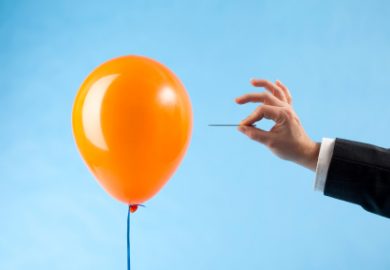
\includegraphics[width=0.8\textwidth]{baloon.png}
    \end{center}
    \begin{flushright}
        \tiny
        \color{gray}from: \url{http://thejobmouse.com}
    \end{flushright}
\end{frame}

\begin{frame}{The Free Desolvation Energy}
    \begin{itemize}[<+->]
        \item Energy needed for transferring atoms from the solvent (water) into
        the protein's interior.
        \item One possible measure of protein stability
        \item The project:
        \begin{itemize}
            \item Implement desolvation energy by \cite{Zhang1997}
            \item Evaluate on \emph{CASP11} data
        \end{itemize}
    \end{itemize}
\end{frame}
% 
% Interaction of atoms keep protein stable
\begin{frame}{Atomic Contacts}
    \begin{center}
        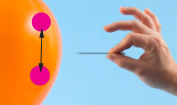
\includegraphics[width=0.8\textwidth]{ace.png}
    \end{center}
    \begin{flushright}
        \tiny
        \color{gray}Based on a picture from: \url{http://thejobmouse.com}
    \end{flushright}
\end{frame}
%
% Model based on atomic contact pairs
% valid if <6A
% 10 bonds away
% picture
\begin{frame}{Atomic Contacts Pairs}
    \begin{center}
        \only<1>{\includegraphics[width=0.8\textwidth]{prot_norm.pdf}}
        \only<2>{\includegraphics[width=0.8\textwidth]{prot_high.pdf}}
    \end{center}
    A valid contact pair:
    \begin{itemize}
        \item Only heavy atoms
        \item Distance below 6\,\AA
        \item More than 10 covalent bonds in between\\
        \uncover<2->{Estimated by connectivity class \& residue index
        differences}
    \end{itemize}
    Overall energy is a simple sum
\end{frame}
%
% 6A limit from packaging
\begin{frame}{Atomic Packaging}
    \begin{center}
        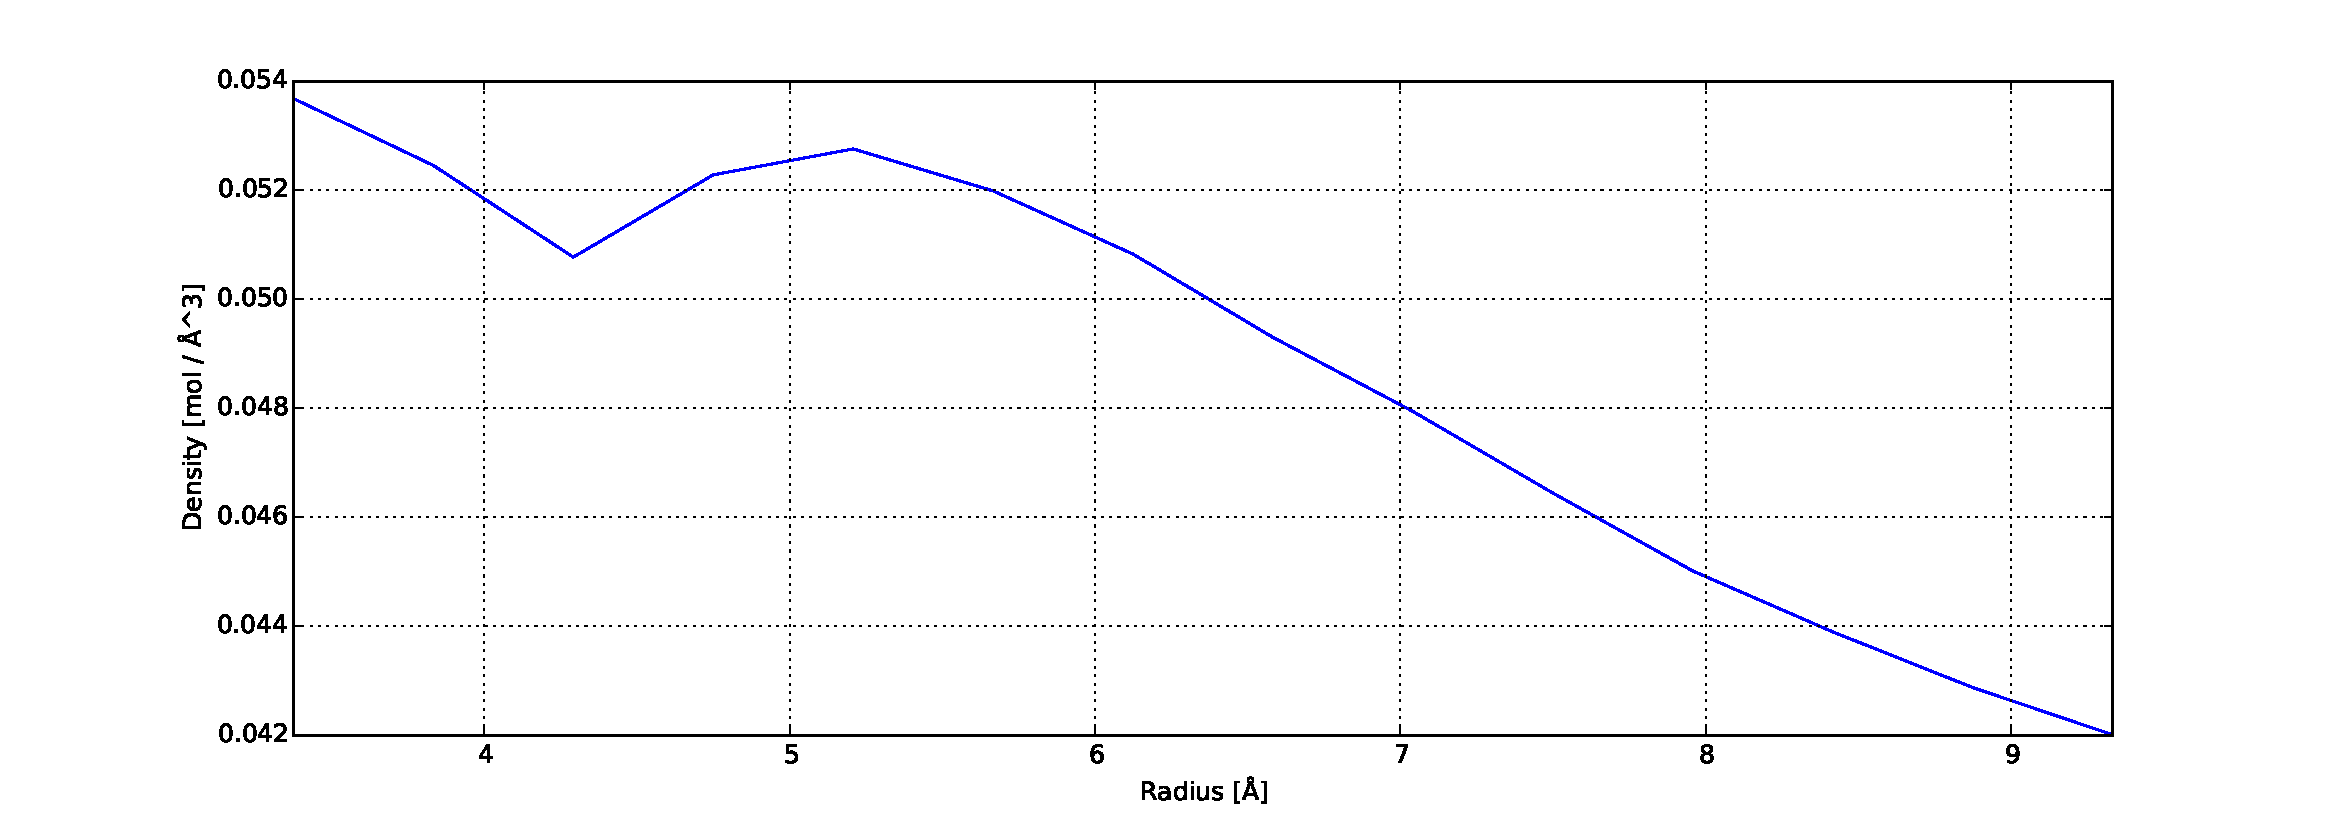
\includegraphics[width=0.9\textwidth]{../results/Density/better.pdf}
    \end{center}

    \begin{itemize}
        \item Number density of interior atoms (SAS = 0)
        \item Relative to a sphere of variable radius
        \item Evaluated on non-homologous protein set
    \end{itemize}
\end{frame}


    \section{Methods}

\colorframe{\ColorMethod}{Methods}
% python + BioPython
% biopython is fast
% lookup of energies stored
\begin{frame}{Implementation}
    \begin{itemize}
        \item Implemented in Python
        \item PDB package from BioPython
        \item Parameters identical to original version
    \end{itemize}
\end{frame}
% evaluated on CASP prediction, beacause quality˜stability
% based on RMSD of CA superimposition (again BioPython)

\begin{frame}{Evaluation}
    \begin{itemize}
        \item Free desolution energy can imply structural stability
        \item Possible measure for Quality for predicted structures
        \item Evaluated on targets of CASP11 competition
        \item Comparison of superimposed $C\alpha$ atoms
    \end{itemize}
\end{frame}

    \section{Results}

\colorframe{\ColorResults}{Results}

\begin{frame}{Comparison with Reference (1/2)}
    \begin{center}
        \begin{minipage}{.45\textwidth}
            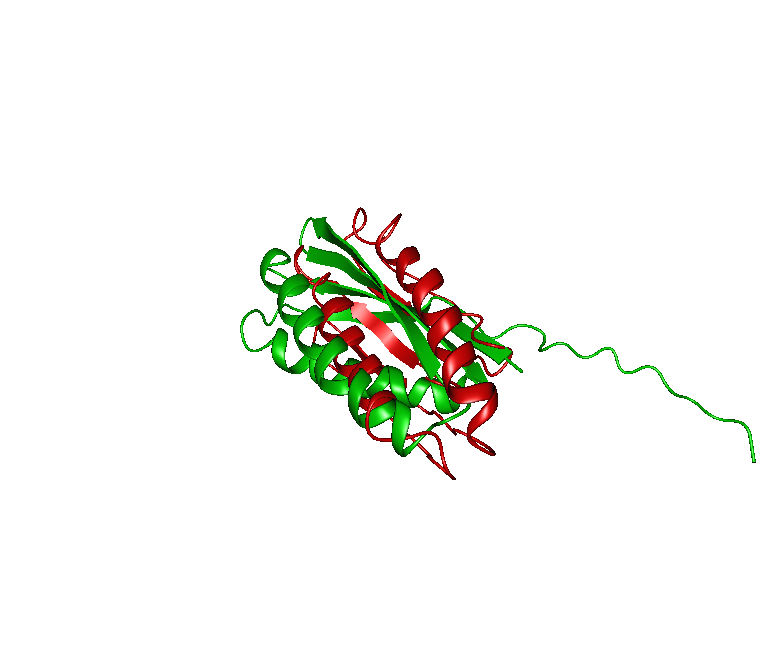
\includegraphics[width=\textwidth]{../report/figures/T0769TS442}\\
            {T0769-442}
        \end{minipage}
        \begin{minipage}{.45\textwidth}
            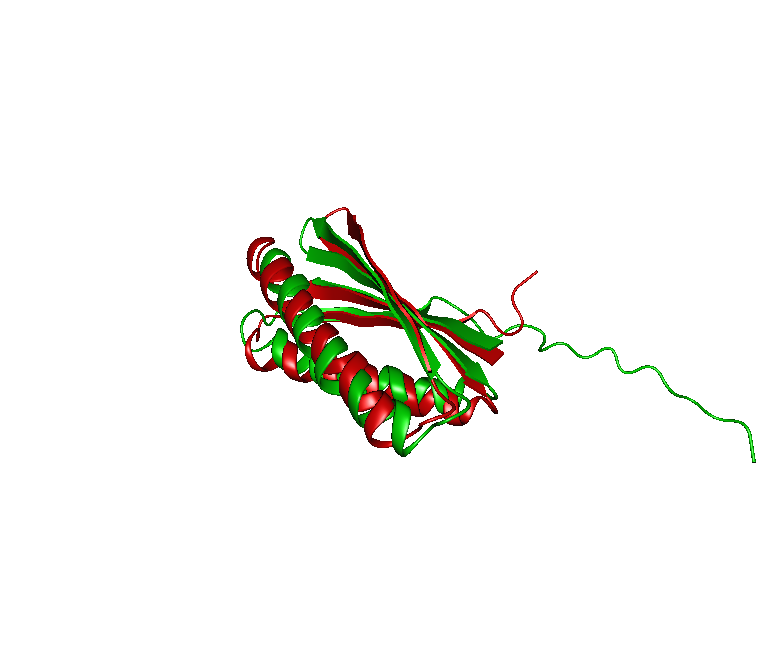
\includegraphics[width=\textwidth]{../report/figures/T0769TS241}\\
            {T0769-241}
        \end{minipage}
    \end{center}
\end{frame}
\begin{frame}{Comparison with Reference (2/2)}
    \begin{center}
        \begin{minipage}{.45\textwidth}
            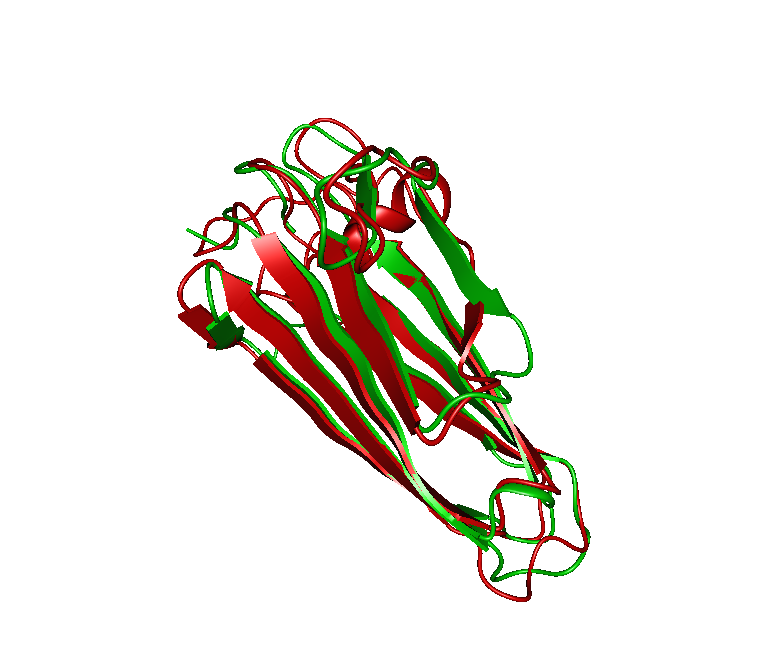
\includegraphics[width=\textwidth]{../report/figures/T0784TS117}\\
            {T0784-117}
        \end{minipage}
        \begin{minipage}{.45\textwidth}
            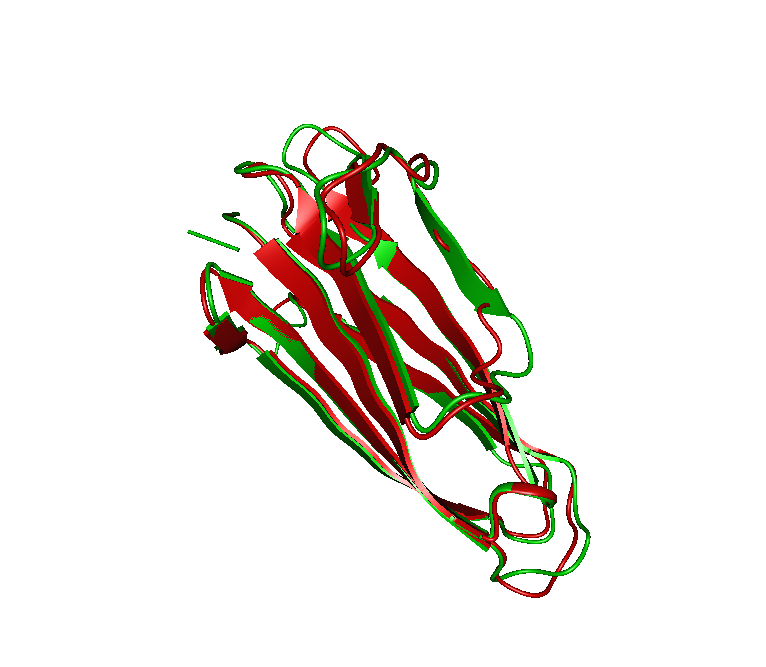
\includegraphics[width=\textwidth]{../report/figures/T0784TS156}\\
            {T0784-156}
        \end{minipage}
    \end{center}
\end{frame}

\begin{frame}{Energy v. RMSD}
	\begin{table}[tbp]
	    \caption{\label{tbl:comparison}For the dataset \texttt{T0784} and
	        \texttt{T0769}, the tables
	        show the computed contact energies and the RMSD counterparts sorted by
	        energies (left) and by RMSD (right).}
	    \scriptsize
	    \centerline{
	        \begin{tabular}{|c|c|c|}
	            \hline
	            \texttt{T0784} & Energy in $\frac{kcal}{mol}$ & RMSD\\
	            \hline
	            T0784TS156\_1 & $-130.48$ & $1.15$\\
	            T0784TS420\_1 & $-127.74$ & $1.17$\\
	            T0784TS499\_1 & $-149.46$ & $1.18$\\
	            T0784TS237\_1 & $-139.99$ & $1.22$\\
	            T0784TS268\_1 & $-160.82$ & $1.28$\\
	            \hline
	        \end{tabular}
	        \begin{tabular}{|c|c|c|}
	            \hline
	            \texttt{T0784} & Energy in $\frac{kcal}{mol}$ & RMSD\\
	            \hline
	            T0784TS117\_1 & $-230.12$ & $1.73$\\
	            T0784TS008\_1 & $-203.16$ & $1.86$\\
	            T0784TS251\_1 & $-193.6 $ & $1.63$\\
	            T0784TS038\_1 & $-162.31$ & $1.38$\\
	            T0784TS268\_1 & $-160.82$ & $1.28$\\
	            \hline
	        \end{tabular}
	    }
	
	    \vspace{2em}
	    \centerline{
	        \begin{tabular}{|c|c|c|}
	            \hline
	            \texttt{T0769} & Energy in $\frac{kcal}{mol}$ & RMSD\\
	            \hline
	            T0769TS241\_1 & $-59.34$ & $2.67$\\
	            T0769TS368\_1 & $-66.75$ & $3.16$\\
	            T0769TS258\_1 & $-74.39$ & $4.37$\\
	            T0769TS361\_1 & $-79.04$ & $4.41$\\
	            T0769TS186\_1 & $-79.97$ & $4.51$\\
	            \hline
	        \end{tabular}
	        \begin{tabular}{|c|c|c|}
	            \hline
	            \texttt{T0769} & Energy in $\frac{kcal}{mol}$ & RMSD\\
	            \hline
	            T0769TS442\_1 & $-90.73$ & $16.72$\\
	            T0769TS155\_1 & $-90.62$ & $17.12$\\
	            T0769TS044\_1 & $-84.32$ & $10.38$\\
	            T0769TS169\_1 & $-81.02$ & $10.39$\\
	            T0769TS317\_1 & $-80.61$ & $ 6.89$\\
	            \hline
	        \end{tabular}
	    }
	\end{table}
\end{frame}

\begin{frame}{Investigation of correlation}
    \begin{center}
        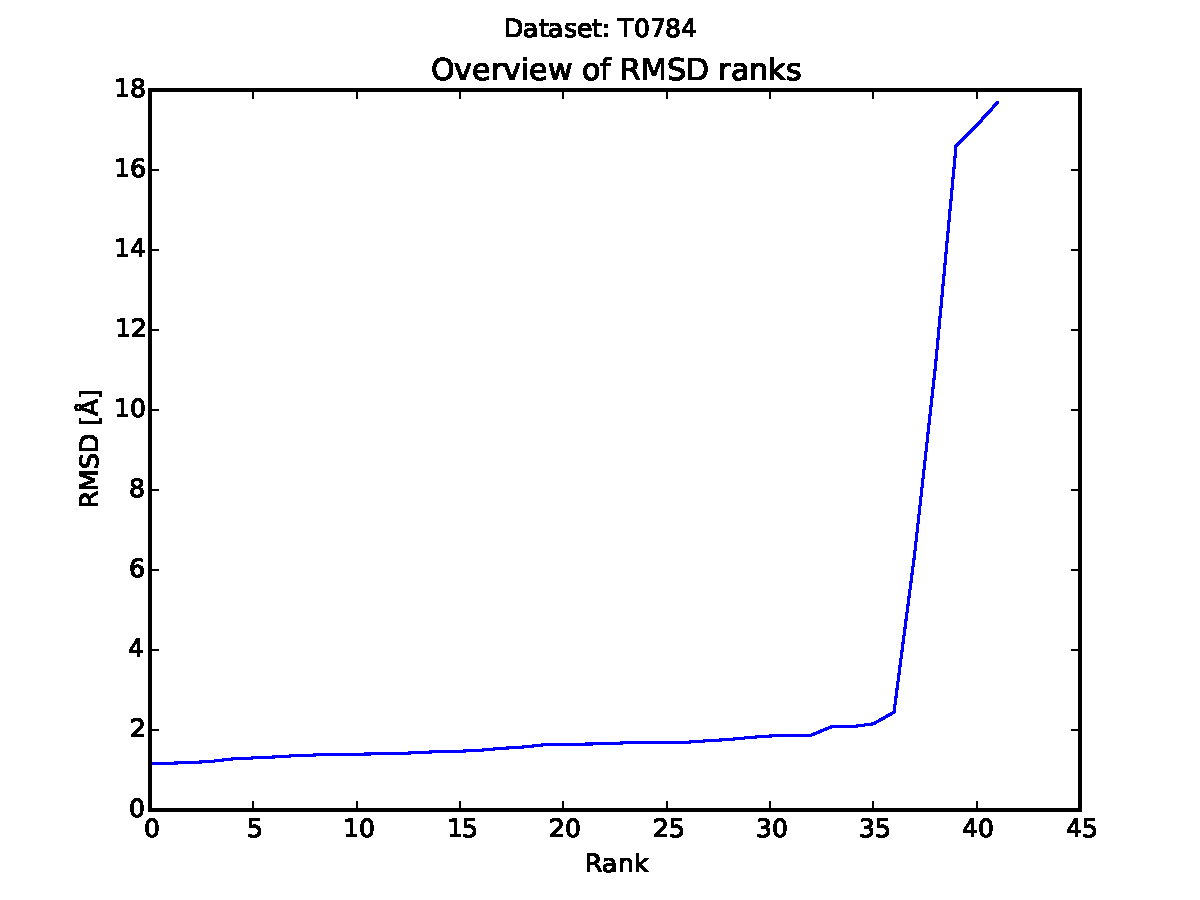
\includegraphics[width=.7\textwidth]{../results/rank_T0784}\\

        \texttt{Pearson}: $0.19-0.44$\\
        \texttt{Spearman}: $0.15-0.33$\\
    \end{center}
\end{frame}

    \section{Conclusion}

\colorframe{\ColorDiscussion}{Conclusion}


% Similarities of Diagrams
% Problems of Correlation
% Problem of RMSD, CASP has many
% Function is fast
% Outperformed aka outdated


    \colorframe{\ColorIntro}{Thank you for your attention!}

    \begin{frame}{Bibliography}
         % References, use smaller font size
        \footnotesize
        \bibliographystyle{jneurosci}
        \bibliography{ref}
    \end{frame}
\end{document}
